\documentclass[../main.tex]{subfiles}
\begin{document}
\subsection*{Exercise 1 – Vehicle model implementation}


\textbf{Q. For each maneuver, plot and comment the main results that you obtain, particularly focusing on tire forces and moments (\{$\fx$, $\fy$, $\fz$, $\mz$\}) and tire slips (\{$\kappa$, $\alpha$\}).}

\begin{enumerate}
  \item initial conditions: $\uz$ = 30 km/h \\
simulation timing: $\ts$\ = 0.001 s, $\tf$\ = 20 s \\
requested pedal: req\_pedal = 1 \\
requested steering wheel angle: req\_steer = 0 deg.
  \end{enumerate}
  
Answer to 1
        \begin{figure}[ht]
        
\includegraphics[width=0.99\linewidth]{ex4/q1/ex-41b.eps}
        \centering
        \caption{vehicle motion graphs}
        \label{41b}
        \end{figure}
        
        
        \begin{figure}[ht]
        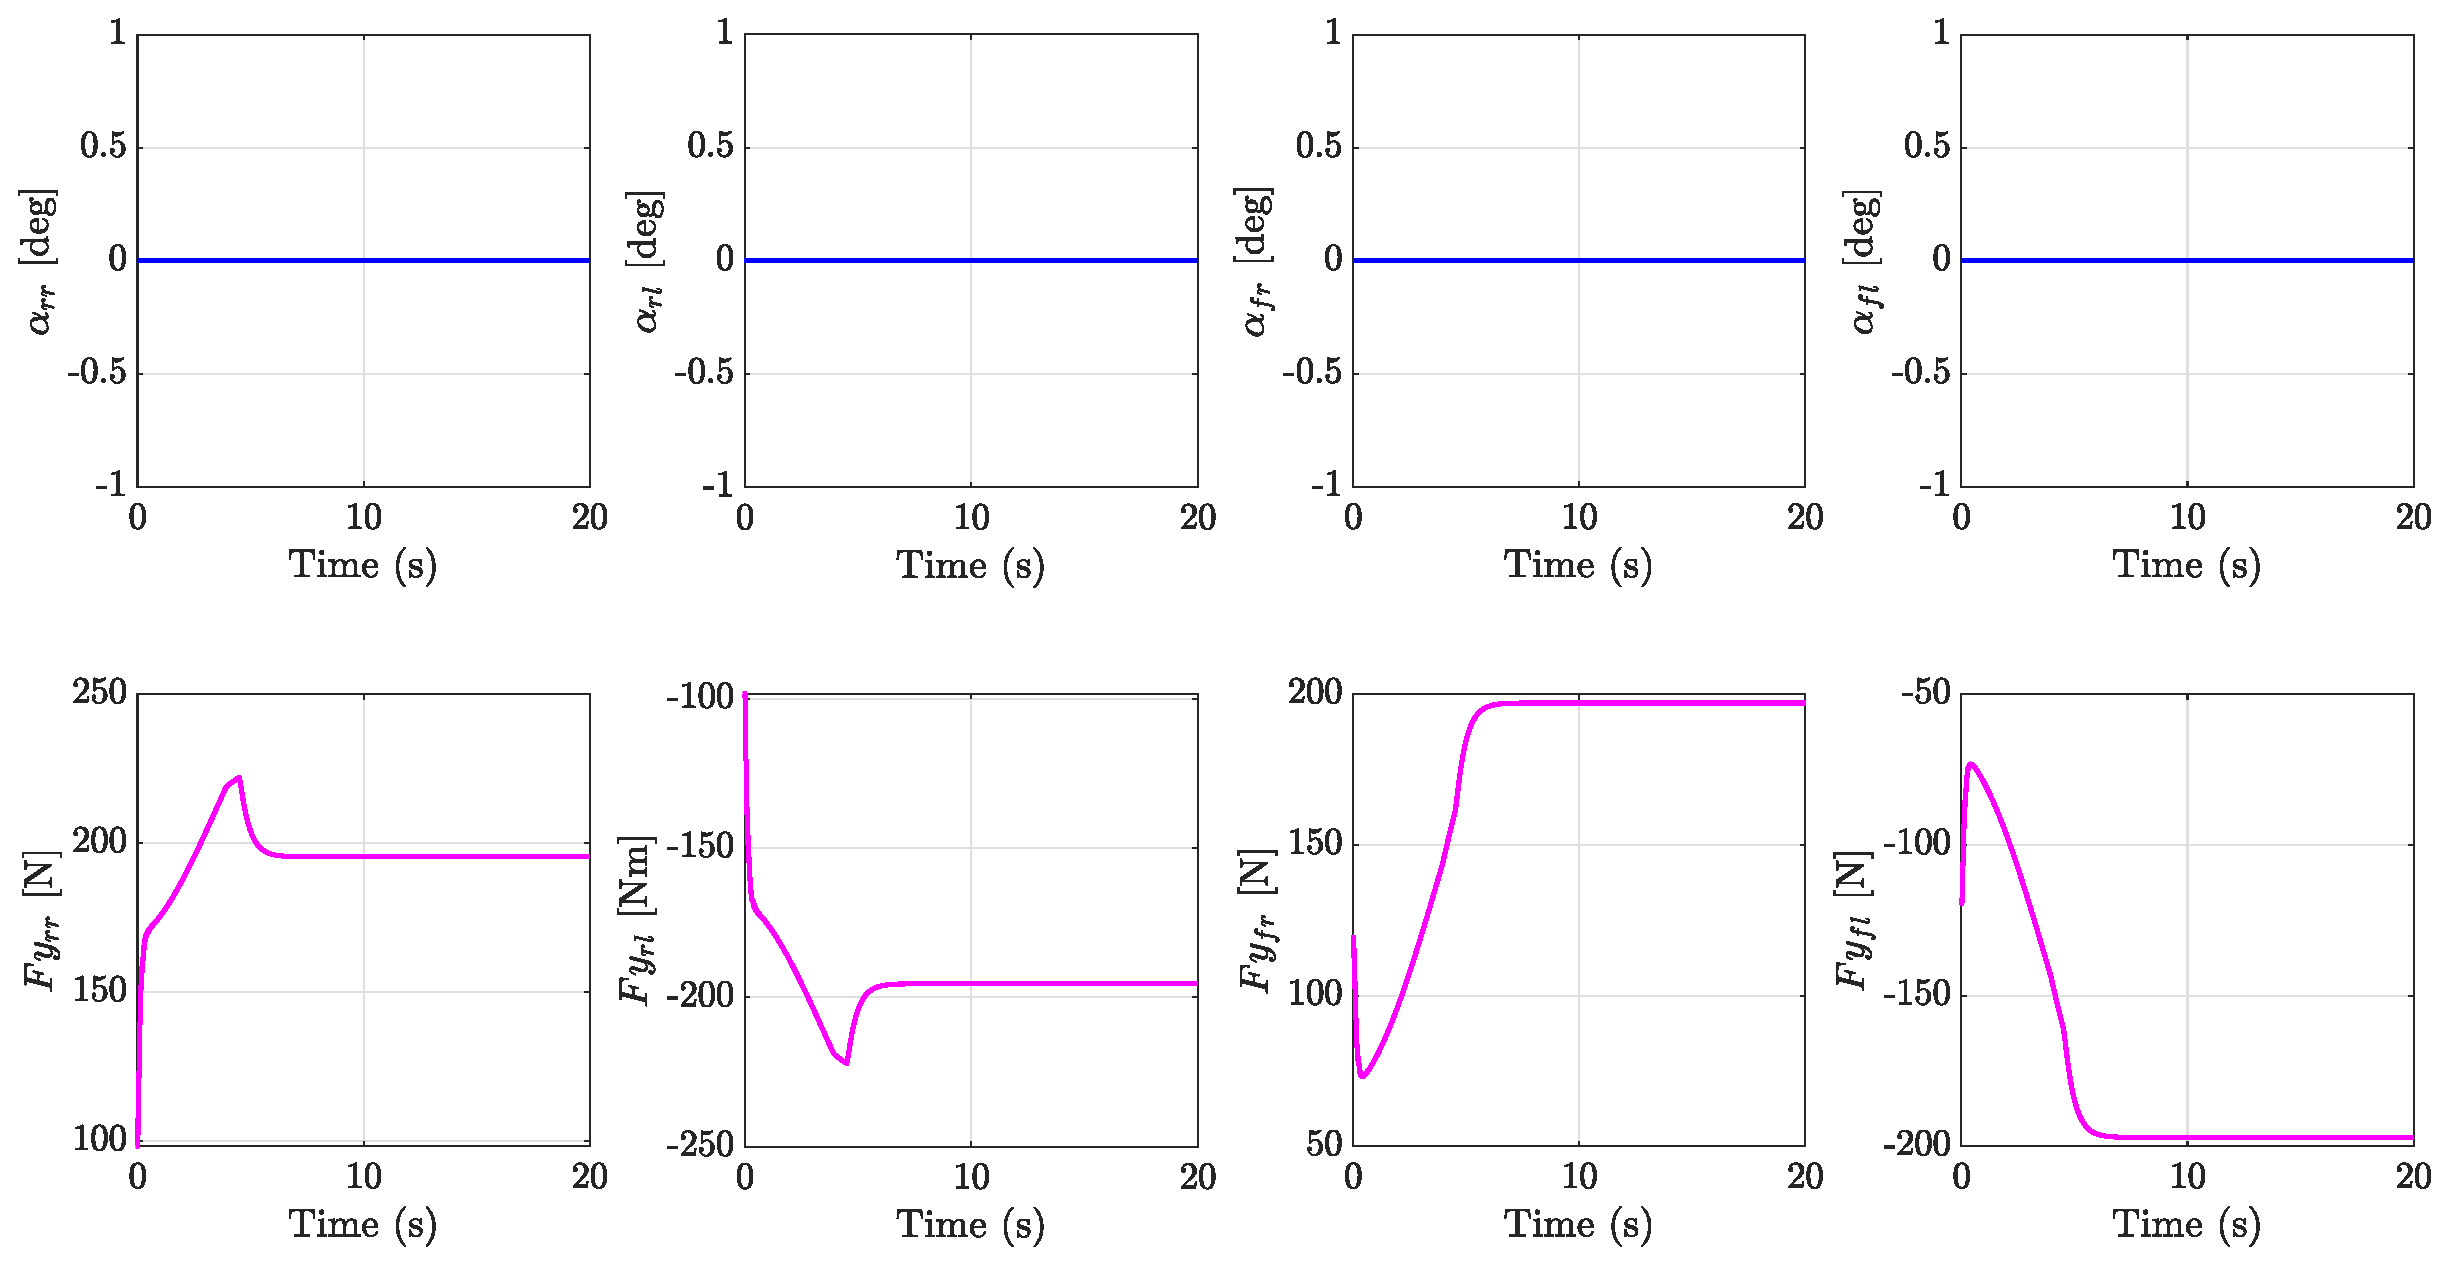
\includegraphics[width=0.99\linewidth]{ex4/q1/ex-41d.eps}
        \centering
        \caption{side slip angle $\alpha$ and lateral forces $\fy$}
        \label{41d}
        \end{figure}
        
        \begin{figure}[ht]
        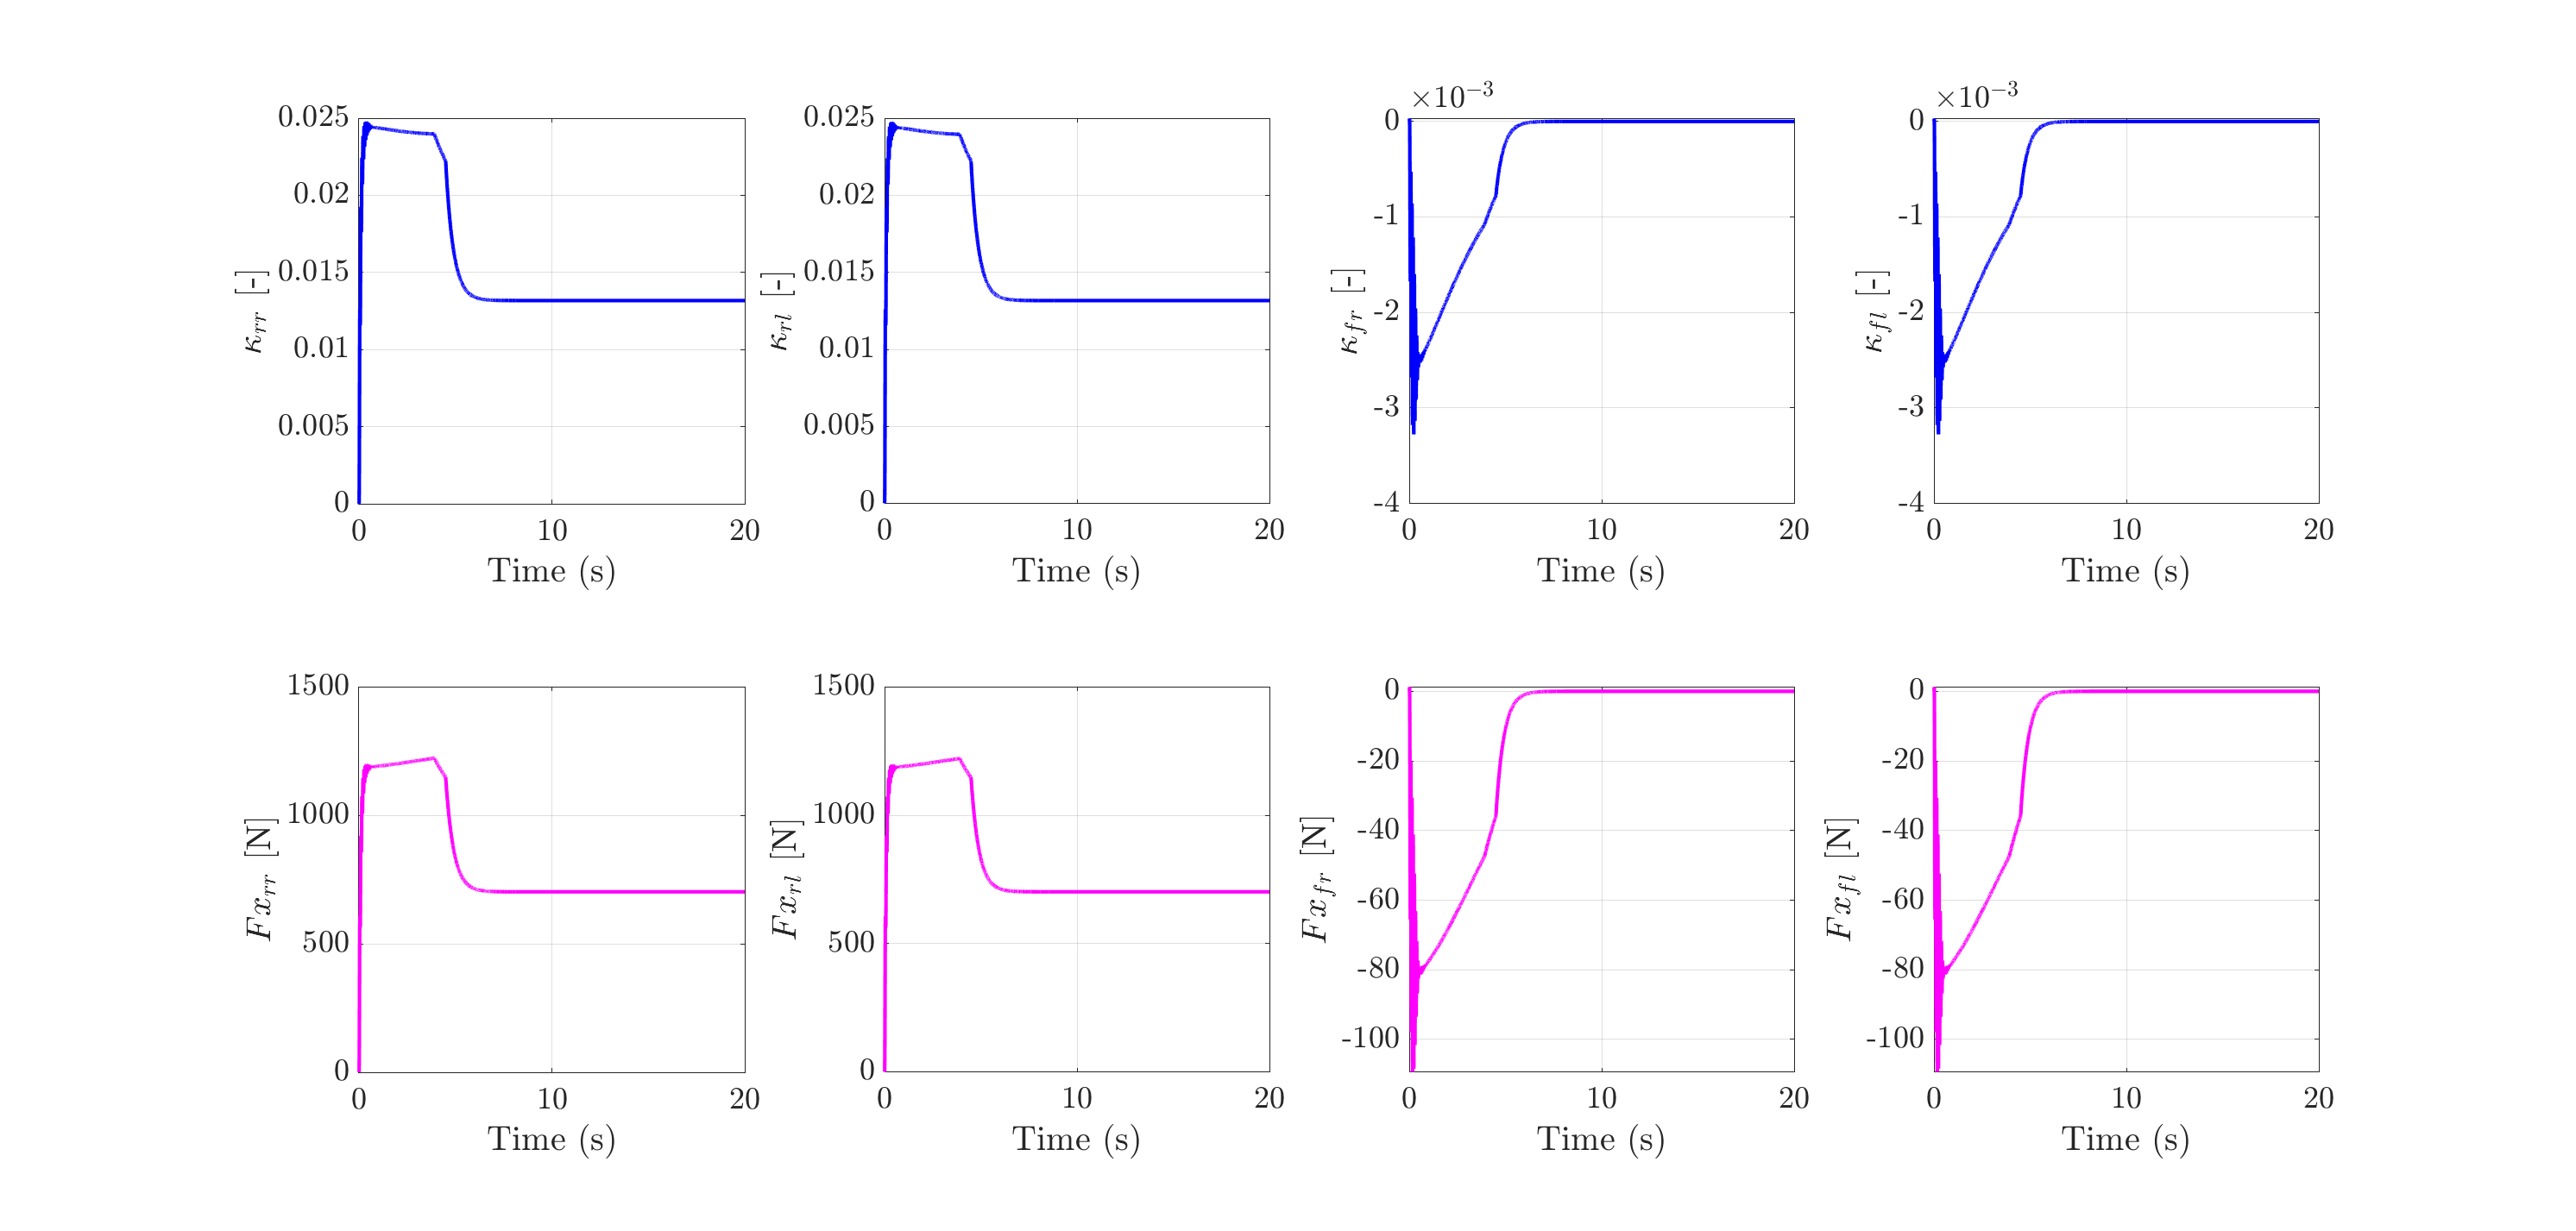
\includegraphics[width=0.99\linewidth]{ex4/q1/ex-41f.eps}
        \centering
        \caption{longitudinal slip $\kappa$ and longitudinal forces $\fx$}
        \label{41f}
        \end{figure}
        
        \begin{figure}[ht]
        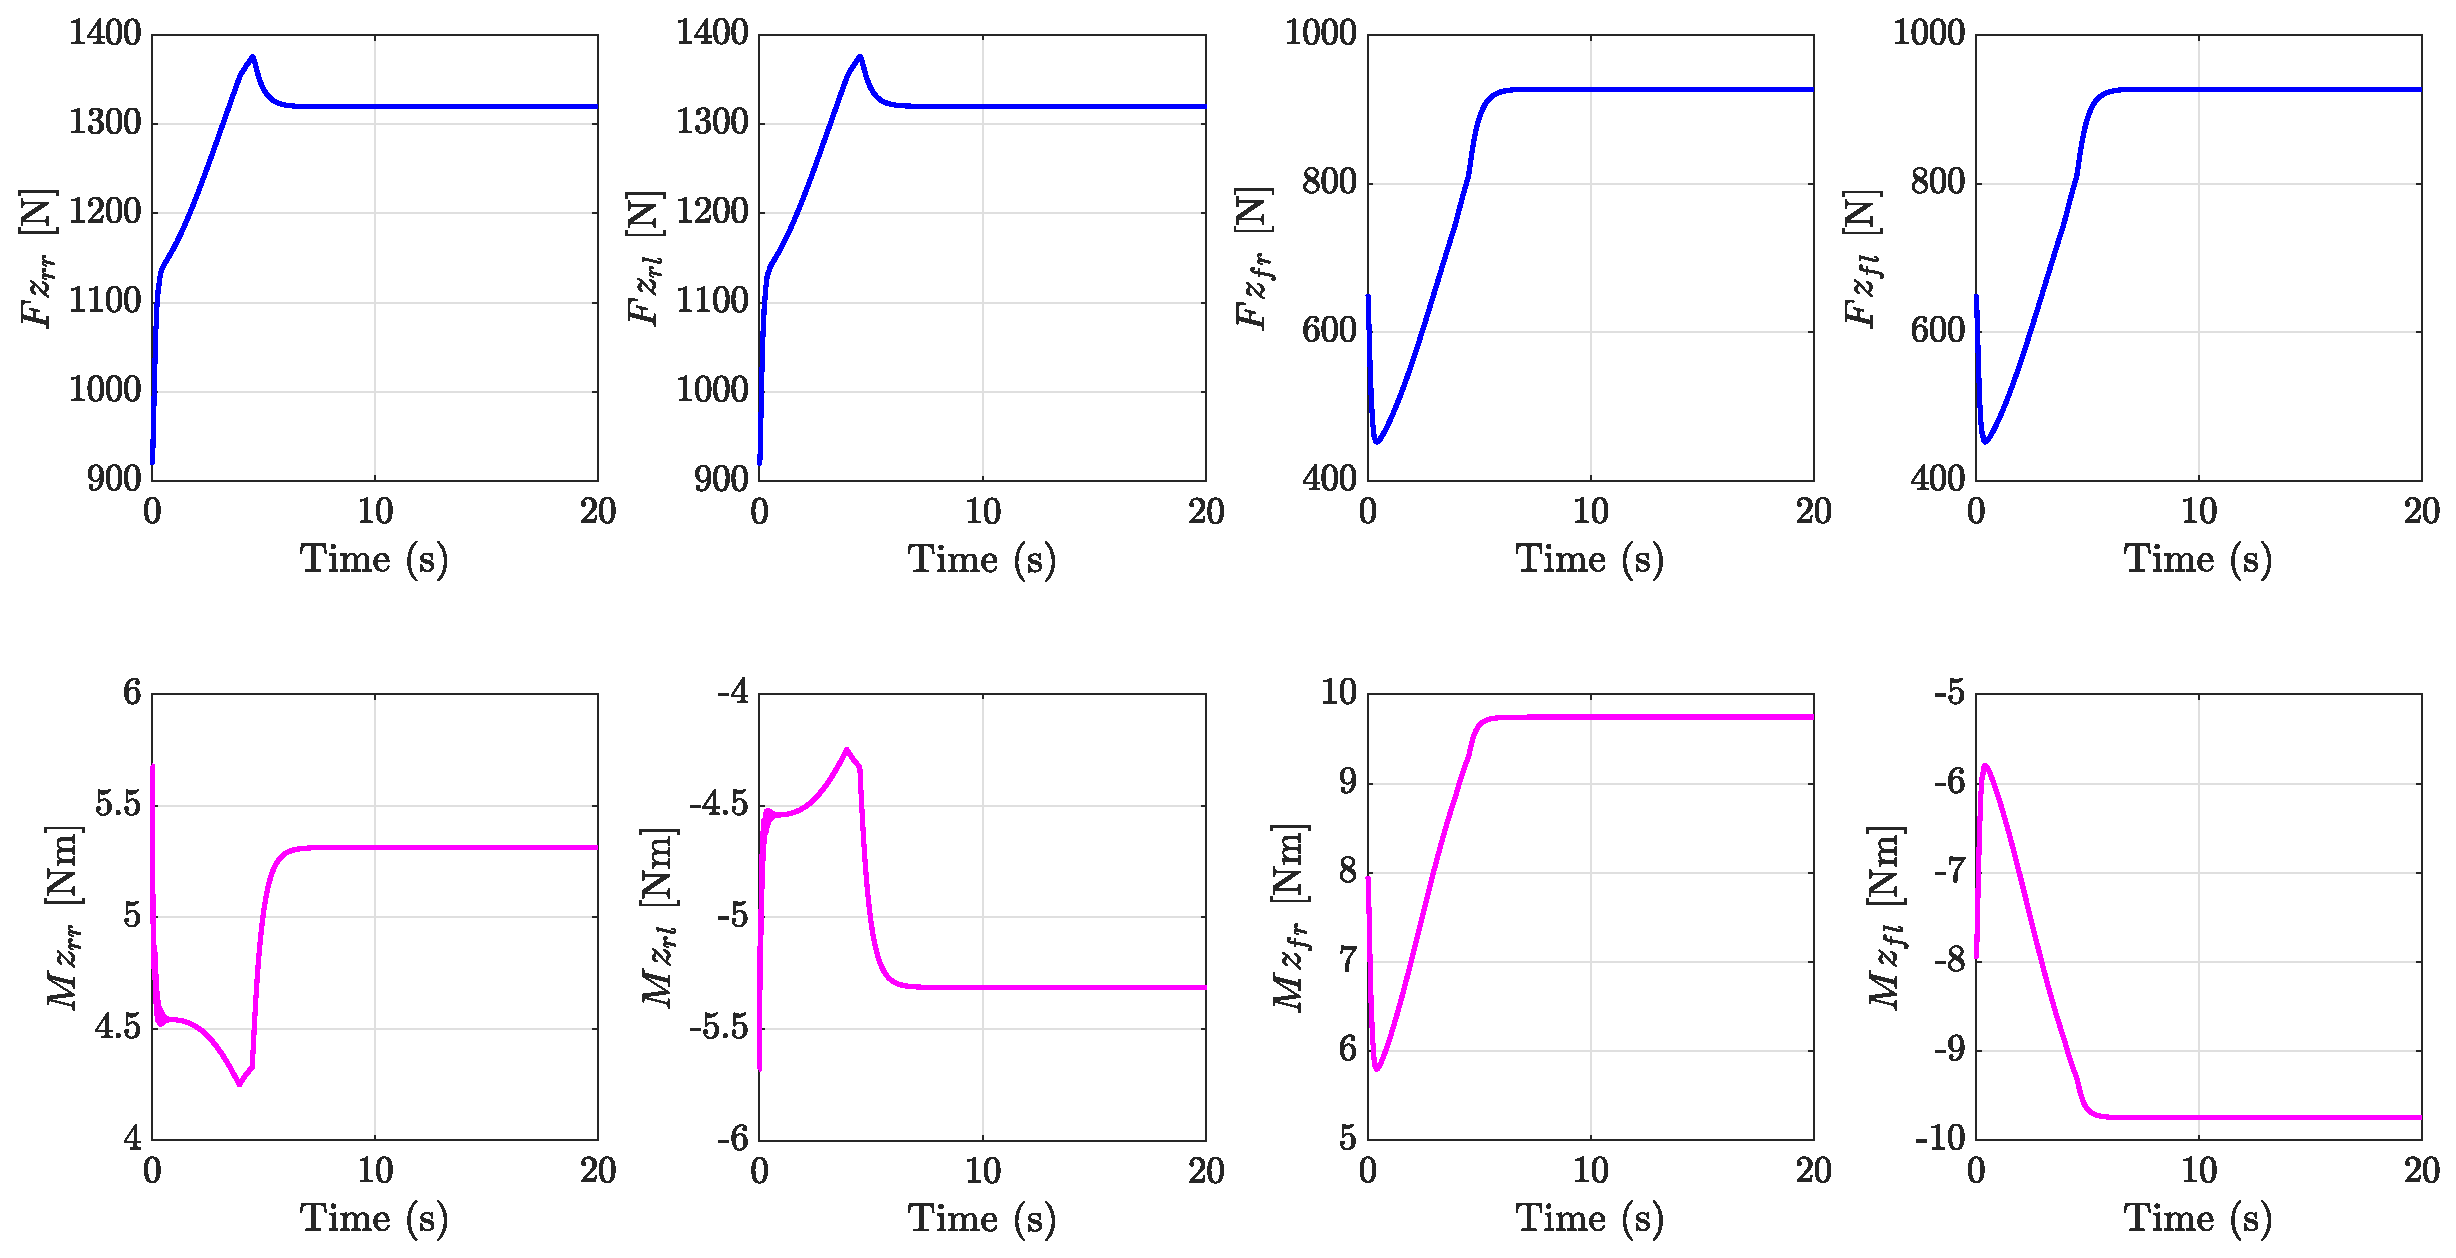
\includegraphics[width=0.99\linewidth]{ex4/q1/ex-41h.eps}
        \centering
        \caption{Vertical forces $\fz$\ and self aligning torque $M_{z}$}
        \label{41h}
        \end{figure}
        
\begin{enumerate}[resume]
  \item initial conditions: $\uz$ = 100 km/h \\
simulation timing: $\ts$\ = 0.001 s, $\tf$\ = 1.5 s \\
requested pedal: req\_pedal = -1 \\
requested steering wheel angle: req\_steer = 0 deg.
  \end{enumerate}

Answer to 2

\begin{enumerate}[resume]
  \item initial conditions: $\uz$ = 50 km/h \\
simulation timing: $\ts$\ = 0.001 s, $\tf$\ = 1.5 s \\
requested pedal: req\_pedal = 0.5 \\
requested steering wheel angle: req\_steer = 20 deg.
  \end{enumerate}

Answer to 3

\end{document}